\cotefile{156-3}
\scanpage{18}\mspage{17}
Sous tronçon \deleted{\illegible{1}}\inserted{fermé $I$} d'un tronçon $\unsure{L|\mathscr{L}}$ : sous ens. de la forme $[a,b]$ (avec $a<b$) ou $L_{\leq a}$ (avec $a$ pas le plus petit élément) ou $L_{\geq\deleted{\unsure{b}}a}$ (avec $b$ pas un plus grand élément), \inserted{ou $L$} : ce sont donc des \unsure{tronçons}, pour la structure de \unsure{biordre|biordonnés|bi-ordre} induite.
\inserted{On a $\partial I=\{a,b\}$ resp $\{a\}$ resp. $\{b\}$, resp $\emptyset$}
% slanted
\margin{Attention il s'agit de frontière \uline{relative} de $I$ dans $L$, et non du bord abs, \unsure{de|abs} $I$.}
\deleted{Donc \unsure{deux} Deux} Deux sous-tronçons fermés sont \deleted{\unsure{disjts|disj.}} en pos. rel. modérée si leurs frontières le sont, i.e. si \unsure{tt|les} \deleted{\unsure{él}} \unsure{point|lieu} frontière de l'un est \unsure{en} pos. rel. modérée à tt \unsure{lieu|point} frontière de l'autre.
\inserted{Sous-tronçon fermé large : soit un sous-tronçon, soit une partie uniponctuelle $\{a\}$, dans ce cas, sa frontière est $a$.}
\deleted{Alors leur int} \deleted{\unsure{est} \unsure{partie}, \unsure{relat.} modérée, \unsure{au cas où}} Deux tronçons fermés larges sont en pos. gén. \deleted{\unsure{sss|ssi}} leurs frontières \deleted{\unsure{donc son} s'il \unsure{le} est en \unsure{pos.} \unsure{gén.} modérée ou si} le sont.
% slanted
\margin{$(I\cap J)^{\unsure{\cdot|\prime|\circ}}\subset I\cup J^{\cdot}$ est vrai par argument topologique,}
Alors leur intersection est vide, \deleted{\unsure{ou un}} ou un \deleted{\illegible{1}} tronçon large, dont la frontière est contenue dans \deleted{\unsure{frontière} \unsure{large en pos. rel. modérée}} la réunion des frontières.
\deleted{\unsure{enfin|afin} \unsure{tt|les} pts frontière. \unsure{qui} \unsure{est} fermés deux tronçon fermé large : tout partie de la}

$\bigl[$\uline{Partie fermée} \uline{modérée} de $I$ : toute partie qui se met sous forme de réunion d'une famille finie de \unsure{ss-tronçons|ss.-tronçons} fermés larges mutuellement disjoints. et mut. \deleted{\unsure{en position}} rel. modérée.$\bigr]$

\unsure{Top.|Tp.} de $L$ \unsure{ici} : Prenant comme base d'ouverts les \unsure{«|``} $]a,b[$ pour $a<b$, et les $L_{>a}$ et $L_{<a}$ \unsure{(}. Alors \deleted{$\unsure{I}$} pour un sous-ps. tronçon \inserted{fermé}, $\partial\unsure{I|\widehat I}$ est la frontière
% slanted
\margin{\uline{NB} Il n'y a pas besoin d'introduire les $L_{>a}$ \unsure{et} si $L$ \unsure{n'a} pas de plus grand élément, et \unsure{itou|idem} pour $L_{<a}$ si \unsure{$a$|$L$} n'a pas de \unsure{plus} petit élément. \unsure{Dans ce cas|Dans} \illegible{2} $]a,b[$ \unsure{eux} \illegible{2} $]a,b[$.}
\scanpage{19}\mspage{18}
\uline{Th} Soit $\unsure{L|\mathscr{L}}$ un tronçon \unsure{biordonné|bien donné}\unsure{;|,} soit $\deleted{\unsure{U}}X\subset L$, tel qu'il existe $I\subset\unsure{\mathrm{Pstrf}|\mathrm{Ps\,tr\,f}}(L)$ (ens des ps-tronçons fermés de $L$), $I$ fini, \deleted{\unsure{formé} de} tel que
\[
\begin{aligned}
\text{a)}\quad \forall i,j\in I,\ i\ne j,\quad
\left\{\begin{aligned}
&T_i\cap T_j=\emptyset\\
&T_i\text{ et }T_j\text{ en pos. rel. mod.}\\
&\text{i.e. }\deleted{\unsure{\partial}}T_i^{\unsure{\cdot|\prime}}\cup \deleted{\unsure{\partial}}T_j^{\cdot}\ \text{\deleted{est} partie}\\
&\qquad\text{finie modérée (ou}\\
&\text{encore }\forall a\in\deleted{\unsure{\partial}}T_i^{\cdot},\ b\in\deleted{\unsure{\partial}}T_j^{\cdot},\\
&a\ne b,\ \text{on a}\quad\{a,b\}\in\underset{\substack{\Vert\\\unsure{\mathrm{Disp}|\mathrm{Dsp}}_2(L)}}{B_{\unsure{0|o}}(L)}
\end{aligned}\right.
\end{aligned}
\]
\deleted{\illegible{1}}
\[
\text{b)}\quad \deleted{U}X=\bigcup T_i
\]

Alors

$1^\circ$) $I$ est \unsure{d'unique|unique} [\unsure{$=$|.} les $T_i$ sont les comp. conn. de $U$]
\margin{NB $U=\emptyset$ sss $I=\emptyset$}
\[
\text{$2^\circ$)}\quad \deleted{\unsure{\partial U|\partial X}}\deleted{U}X^{\cdot}=\bigcup_{i\in I}T_i^{\cdot}
\]
\[
(\text{donc }\deleted{U}X^{\cdot}=\emptyset\quad\text{sss}\quad\deleted{\unsure{I=\emptyset\ \text{ou}}}\quad\deleted{U}X=L\text{ ou }\deleted{U}X=\emptyset
\]
(On dit que $\deleted{\unsure{U}}X$ est une \uline{partie} \uline{modérée}) \uline{fermée}.

\uline{Def} Si $\deleted{U}X,\deleted{\unsure{V}}Y$ sont deux parties \uline{fermées} modérées, on dit que $X$ et $Y$ sont en pos. \unsure{relative|relation} modérée $X^{\cdot}$ et $Y^{\cdot}$ le sont, i.e
\[
\forall x\in X^{\cdot},\ y\in Y^{\cdot},\ \inserted{\text{avec }}\unsure{a|x}\ne y,\ \text{on a }\{x,y\}\in\mathrm{Disp}_2
\]
% margin note written sideways
\margin{\uline{Ex} Si $X$ et $Y$ sont \unsure{modérées|modérés}, avec $X\subset Y$, alors $X^{\cdot}\unsure{\subset|\in}Y$ donc tt pt de $X^{\cdot}$ est en pos. rel. modérée par \unsure{$X$ et $Y$} (\unsure{i.e.|lire} \unsure{p.r. à} $Y^{\cdot}$) \unsure{donc} \unsure{sont|sont en} en pos. modérée.}
\scanpage{20}\mspage{19}
% slanted
\margin{partie de \deleted{\unsure{Th}} \unsure{th.}}
\deleted{\uline{\unsure{Prop}}}\inserted{\uline{Prop} Soit $X,Y$} Deux parties fermées modérées, \unsure{en} pos. rel. modérée. Alors $X\cap Y$ est une partie \inserted{fermée} modérée, et
\[
\boxed{(X\cap Y)^{\unsure{\cdot|\prime}}\subset X^{\cdot}\cup Y^{\cdot}}
\]
De plus, \inserted{$X$ et $Y$ ont une borne sup. \unsure{dans|en}} \deleted{\unsure{parmi} \unsure{toutes les} parties} l'ens des parties modérées ordonnées par \deleted{fermées modérées qui \unsure{contient} $X$} l'inclusion.
% slanted
\margin{\deleted{\unsure{Dém}} \uline{Dém} double récurrence sur nb de comp. conn. de $X$ et de $Y$ (pour l'existence du \unsure{Sup|sup} et la \unsure{question des frontières})}
\deleted{$X$ et $Y$, et on} On écrit cette partie $X\underset{\mathrm{mod}}{\cup}Y$, On a
\[
\boxed{(X\underset{\mathrm{mod}}{\cup}Y)^{\cdot}\subset X^{\cdot}\cup Y^{\cdot}}
\]
% slanted
% Two nearly parallel strokes separate the left notes, immediately above Rem.
\margin{Rem, \unsure{tte} partie modérée $Z$ en pos. rel. \unsure{mod.} avec $X$ et $Y$, l'est aussi avec $X\cap Y$ et $X\underset{\mathrm{mod}}{\cup}Y$}

\uline{Cor} Soit $(X_i)_{i\in I}$ une famille finie de \unsure{partie|parties} fermées modérées mutuellement en pos. \deleted{rel} modérée. Alors $\bigcap_i X_i$ est une partie modérée, et les $X_i$ ont une borne sup. \unsure{ds|dans} l'ens des parties fermées modérées. On a
% slanted
\margin{\uline{Attention} pour une partie \uline{\unsure{quelc|seule}} $A$ de $\unsure{L|\mathscr{L}}$, il n'y a \uline{pas} en général d'\unsure{adh.} modérée fermée, i.e. de ``plus petit'' ens \unsure{f.} modéré $X$ tel que $X\supset A$. C'est déjà faux ds le cas standart $L=[0,1]$ ! (Prendre $A=\{\unsure{0|1},1/2,1/3\ldots\}$}
\[
\left(\bigcup_{\substack{\mathrm{mod}\\ i}} X_i\right)^{\cdot}\subset\bigcup_i X_i^{\cdot}
\]

\uline{Ex}
\[
[a,b]\underset{\mathrm{mod}}{\cup}[b,c]=[a,c]
\]
mais en général
\[
[a,b]\cup[b,c]\ne[a,c]
\]
(\unsure{prendre|quand} $a$ plus \unsure{c|e} petit élément, $c$ plus grand élément \deleted{\unsure{et}} \unsure{qqconq} \deleted{\unsure{Et en ce} $\unsure{=}$}, $b$ \deleted{\unsure{est}} comp. à tout \inserted{élément de $L$.} Si c'est
\scanpage{21}\mspage{20}
vrai pour tt $b$, alors $\unsure{L|\mathscr{L}}$ est \unsure{ttt|tt} ordonné. Plus \unsure{précisém$^{\mathrm t}$|précisément|généralem$^{\mathrm t}$}, pour que $L$ ttt ordonné, il f et s. que pour tt $b\in L$, $b$ soit comparable à tt autre élément, ce qui s'écrit
\[
\underbrace{L_{\leq b}\underset{\mathrm{mod}}{\cup}L_{\geq b}}_{L}=L_{\leq b}\cup L_{\geq b}
\]
\begin{center}\rule{2.5cm}{0.35pt}\end{center}

Partie loc. fermée modérée

\uline{Th} Soi\deleted{\unsure{ent}}t $X\deleted{\unsure{\subset|\supset}},Y$ deux parties fermées modérées, avec $X\supset Y$ (donc $X$ et $Y$ en pos. relative modérée)
\deleted{Considérons les} \deleted{Alors $\exists$ une plus petite partie fermée modérée \inserted{$Z$} contenant $X\setminus Y$.}
Soit
\[
\deleted{\unsure{\complement_X|C_X|\partial X}} C_{\mathrm{mod}}(Y,X)=\left\{x\in X\ \middle|\ 
\begin{aligned}&x\notin Y,\ x\text{ en pos. rel.}\\[-2pt]&\hphantom{x\notin Y,\ x\text{ en }}\text{mod. avec }Y\end{aligned}\right\}
\]
Alors $\exists$ plus petit ens. fermé modéré $Z$ \deleted{tel} \inserted{\unsure{contenant}} \deleted{\unsure{tt|te}} $C_{\mathrm{mod}}(Y,X)$, \deleted{\unsure{a}}\inserted{Ce} $Z$ \inserted{est $\subset X$, et} contient \deleted{\unsure{tt}} partie fermée modérée $T$ de $L$ telle que $T\subset X$, $T\cap Y=\emptyset$, $T$ en pos. rel. mod par. \inserted{\unsure{rapt|rel.}} à $Y$, \inserted{\unsure{De plus}} $Z$ est en position modérée avec $Y$.
% slanted
\margin{\uline{On pose} $Z=X\underset{\mathrm{mod}}{\setminus}Y$}
\scanpage{22}\mspage{21}
Si on pose $\deleted{\unsure{S|J}}F=$ frontière relative de $Y$ dans $X$, \deleted{\unsure{c.} F} Alors $F$ est fini, \inserted{modéré,} en pos. mod. \unsure{p.r.} à $Y$, \deleted{\unsure{dans}} $F\subset Z$, \deleted{$\unsure{F\cap Z}$} \deleted{\unsure{est}} $F$ ne \deleted{$\unsure{Z}$} contient pas de pts isolé de $Z$.
\deleted{et on a}
\[
\deleted{\unsure{\mathrm{Comp}}}\ C_{\mathrm{mod}}(Y,X)=C_{\mathrm{mod}}(\deleted{\unsure{Z}}F,Z)
\]
\figure{\tikz{\draw (0,0) .. controls (.07,.02) and (.15,.10) .. (.21,.08) .. controls (.24,-.03) and (.38,-.01) .. (.55,.04) .. controls (.70,.11) and (.74,-.04) .. (.90,-.04) .. controls (1.22,-.05) and (1.33,.05) .. (1.48,.05) .. controls (1.66,-.04) and (1.78,-.08) .. (1.95,-.06) .. controls (2.16,-.05) and (2.27,.08) .. (2.41,.05) .. controls (2.56,-.05) and (2.81,-.05) .. (3.04,.00) .. controls (3.20,.02) and (3.32,.12) .. (3.42,.06) .. controls (3.50,-.08) and (3.80,-.02) .. (4.10,-.01);}}

(9 juin) Soit $\unsure{L|\mathscr{L}}$ un tronçon ordonné.

\deleted{Un sous-segment \unsure{d'un|dans} \uline{sous-tronçon} \uline{fermé} de $L$ est un sous ens de la forme $[a,$}

\textcircled{1} Topologie sur $L$ : base d'ouverts les $]a,b[$ (pour $a<b$), $L_{<a}$\deleted{\unsure{,}}, $L_{>b}$
[NB si $L$ n'a pas de plus petit élément (resp. de plus grand élément) on peut \unsure{omettre} les $L_{<a}$ (resp. les $L_{>b}$). \inserted{\unsure{Une} extrémité de} \deleted{Pour que $\unsure{\{a\}}$ soit} $L$ \unsure{—|(} (s'il y en a) est fermé, mais \deleted{fermé, il f et \unsure{suff} s. que}
On fera attention qu'en général, \deleted{les $\unsure{\{a\}}$} \deleted{\unsure{si $a$ est|si $a$ et}} pour $a\in L$ $\{a\}$ \uline{n'est pas} \inserted{\uline{\unsure{néct|néct$^{\mathrm t}$}}} \uline{fermé}. Si $L$ est l'ens des lieux d'une \deleted{\unsure{segm}} ficelle topologique\unsure{$^{x}$|,}, \deleted{et} alors $\deleted{\unsure{a}}b\in\overline{\{\deleted{\unsure{b}}a\}}$ i.e. $\overline{\{b\}}\subset\overline{\{a\}}$, équivaut à $b\supset a$ (en tt que parties de \unsure{$\mathscr H$|$\mathcal H$|$H$})
\scanpage{23}\mspage{22}
Il en résulte que $\overline{\{\deleted{\unsure{b}}a\}}=\overline{\{b\}}\Longleftrightarrow a=b$ \unsure{(donc|donc|Alors} l'espace top $\unsure{L|\mathscr{L}}$ satisfait l'axiome $T_0$, il est ``présobre'' i.e. s'injecte \unsure{dans|ds} le présobrifié) -- je ne sais si c'est
le cas pour tout tronçon, \unsure{ni|ni même} si un tronçon, avec sa top. canonique, est sobre (donc, de plus, tte partie fermée \uline{irréductible} aurait un pt générique \dots)
% A step-shaped double vertical stroke joins the underline above to the end of the preceding line.
\margin{\unsure{A|À} voir\unsure{.|,}}
les ``\unsure{segment|segments}'' $[a,b]$ ne sont pas néc. fermés pour la top. canonique\unsure{$^{\dagger}$|$^{+}$|!}\unsure{,|.}
Ce n'est que lorsque $L$ est \uline{tot} ordonné qu'on peut conclure que les pts sont fermés (réciproque ?) et en fait, $L$ est $\unsure{=|\simeq}$ \uline{séparé}, et de plus les $[a,b]$, $L_{\geq a}$, $L_{\leq\deleted{\unsure{b}}a}$ sont fermés.

On peut définir une autre topologie, ayant comme base fondamentale de fermés les $[a,b]$, $L_{\geq a}$, $L_{\leq a}$ (dont on prend les intersections \unsure{quelc\textsuperscript{on}|quelc.} de réunions finies, pour avoir tous les fermés)
\scanpage{24}\mspage{23}
Mais maintenant, on est \unsure{ennuyé}, car $]a,b[$ n'a plus envie d'être ouvert !

\deleted{\unsure{ici|on}} On peut bien sûr prendre la topologie borne sup. des deux, ayant comme base d'ouverts

\[
\begin{aligned}
 \unsure{L|\mathscr{L}}_{<a},\,L_{>a},\quad &]a,b[ && (a<b)\\
 \complement L_{\deleted{\unsure{\leq|>}}\geq a},\,\complement L_{\leq a},\quad &[a,b] && (a<b)
\end{aligned}
\]

\deleted{De sorte que $]a,b[$ \unsure{est|est un}} \deleted{Sera-t-il vrai, si $a\unsure{\nless|\leq|<}b$, et} \deleted{Mais} \deleted{$b$ n'est pas plus grand élément, que}

Aura-t-on \deleted{$b\in [a,b$}
\[
\begin{aligned}
 \overline{]a,b[}&=[a,b]\quad ?\\
 \overline{L_{<a}}&=L_{\leq a}\quad ?\quad \text{(si $a$ \deleted{\unsure{n'|est}} n'est pas plus petit élément\unsure{—|)}} \quad \inserted{(a\ne\unsure{o|0}_{L})}\\
 \overline{L_{>a}}&=L_{\geq a}\quad ?\quad \text{(si $a$ n'est pas plus grand élément ?)}
\end{aligned}
\]

\figure{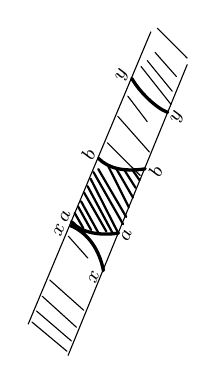
\begin{tikzpicture}[rotate=67,x=.84cm,y=.84cm,line cap=round,line join=round,every node/.style={transform shape,inner sep=1pt,font=\scriptsize}]\draw (.20,.74)--(4.99,.76) (0,0)--(4.75,.06);\draw[thin] (.05,.04)--(.25,.70) (.22,.04)--(.43,.70) (.44,.05)--(.67,.71) (.72,.05)--(.94,.70) (1.47,.30)--(1.66,.70) (2.93,.06)--(3.19,.71) (3.31,.07)--(3.62,.72) (3.72,.28)--(3.96,.70) (4.10,.05)--(4.45,.69) (4.29,.11)--(4.57,.64) (4.52,.14)--(4.73,.58) (4.84,.10)--(5.08,.69);\draw[very thick] (1.39,.01) .. controls (1.64,.18) and (1.82,.43) .. (1.82,.73) (2.00,.02) .. controls (1.85,.26) and (1.78,.55) .. (1.88,.74) (3.05,.03) .. controls (2.88,.31) and (2.84,.54) .. (2.92,.74) (3.97,.05) .. controls (3.96,.23) and (4.08,.55) .. (4.23,.75);\draw[thick] (1.86,.54)--(2.02,.75) (1.88,.42)--(2.13,.74) (1.89,.31)--(2.22,.73) (1.95,.20)--(2.36,.74) (1.97,.11)--(2.47,.73) (2.01,.04)--(2.59,.73) (2.15,.01)--(2.70,.73) (2.27,.01)--(2.77,.68) (2.42,.03)--(2.87,.56) (2.58,.03)--(2.88,.43) (2.73,.05)--(2.91,.31) (2.86,.04)--(2.96,.20);\node[above] at (1.69,.75) {$x$};\node[above] at (1.92,.75) {$a$};\node[above] at (2.91,.75) {$b$};\node[above] at (4.22,.76) {$y$};\node[left] at (1.38,.10) {$x$};\node[below] at (2.01,.01) {$a$};\node[below] at (3.07,.02) {$b$};\node[below] at (3.96,.03) {$y$};\end{tikzpicture}}
\deleted{\unsure{Donc|D'où}} On est ramené, dans le premier cas, à prouver (p. ex.) $a\in\overline{]a,b[}$, et pour ceci, \inserted{il suffit de voir} \deleted{\unsure{On|que}} que \unsure{tt|tte} ouvert ``élémentaire'' qui contient $a$, contient un $]a,\varepsilon[$, avec $a<\varepsilon<b$. Mais c'est faux déjà pour un ens. de lieux associé à une ficelle topologique, \deleted{\unsure{en}} [prendre ouvert él. $\complement[x,y]$\unsure{—|.}

% slanted
\margin{Il \unsure{faut avoir|faudrait avoir} que $a\in\complement[x,y]$ mais $]a,b[\,\subset [x,y]$}
\scanpage{25}\mspage{24}
Finalement, on travaillera avec la top. définie d'abord (base formée avec les ``intervalles''), et on appellera néanmoins par abus de langage, les $[a,b]$, $\unsure{L|\mathscr{L}}_{\leq a}$, $L_{\geq b}$ (ainsi que $L$) \uline{sous-tronçons} ordinaires (ou \unsure{biordonnés|bien donnés|bien disons|binominés}) ``fermés'', [NB on les suppose \unsure{non|ici} réduits à un pt, i.e.
\[
\deleted{\unsure{[|i}} a<b\quad \text{resp.}\quad a\ne\mathrm{or}(L)\quad \text{resp.}\quad \deleted{\unsure{a}}\unsure{b|a}\ne\mathrm{ex}(L)\;]
\]

Un \uline{sous-tronçon \inserted{fermé} large} est une \deleted{sous-tronçon} partie qui est soit un \unsure{ss-tronçon|s-tronçon}, soit \unsure{réduit|réduite} à un pt.

Pour une telle partie, $T$, on
% Widely spaced strokes cross the whole lower block, from pose to the last example.
% The close zigzags and local horizontal cancellations show an earlier level of correction.
\deleted{pose}
\[
\begin{aligned}
\deleted{\partial T=}&\deleted{\{t\in T\mid t\in \overline{L\setminus T}\}}\quad\text{\deleted{bord}}\\
 &\text{\deleted{\unsure{frontière dans la top.|frontière dans la top}}}\\
 &\text{\deleted{absolu de $T$ $=$ ensemble}}\\
 &\text{\deleted{\unsure{canonique}}}\\
 \deleted{={}\unsure{T\cap L|T\cap\overline{L}}}&\quad\text{\deleted{fermé de ses extrémités}}\\
 &\deleted{(\mathrm{NB}\ \mathrm{card}\,\partial T\in\{0,1,2\})}
\end{aligned}
\]

\deleted{On voit que pour un tronçon fermé (\uline{NB} non réduit à un pt) on a}

\[
\begin{aligned}
 \deleted{\partial[a,b]=\{a,b\}}&\qquad \deleted{\partial L_{\leq a}=\{a\},\quad \partial L_{\geq a}=\{a\}}\\
 &\deleted{\partial L=\emptyset}
\end{aligned}
\]
